%\documentclass[a5paper, 10pt, twoside, openany]{book}
\documentclass[fontsize=9pt,paper=a5,footinclude,headinclude, twoside, final]{scrbook} % KOMA-Script book
\usepackage[cmyk,hyperref,dvipsnames]{xcolor} %The two first options are for pdf-x, the last is for classicthesis

\usepackage[pdfpagelabels, unicode, pdfstartview=FitH]{hyperref}
\usepackage[swedish,british]{babel}
\usepackage{url}
\usepackage{iftex}

\ifLuaTeX
	\usepackage{luatextra}
	\usepackage{fontspec}
\else
	\usepackage[utf8]{inputenc}
	\usepackage[T1]{fontenc}
\fi

\usepackage{graphicx}
\usepackage{caption}
\usepackage{subcaption}
\usepackage{bibentry}

\usepackage[centertags]{amsmath}
%\usepackage{amsfonts}
\usepackage{amssymb}
\usepackage{amsthm}
\usepackage{amsmath}
\usepackage{siunitx}
\usepackage{fancyvrb}
\usepackage{lettrine}

% Remove indentation in bulletpoints
\usepackage{enumitem}
\setlist{leftmargin=0mm}

\ifLuaTeX
	\usepackage[math-style=french]{unicode-math}
\fi

\usepackage[eulerchapternumbers=true, eulermath=true, parts=true, floatperchapter]{classicthesis}
\usepackage[paperwidth=165mm, paperheight=242mm, outer=40mm, inner=20mm, marginparwidth=25mm, top=20mm]{geometry}
%\usepackage[paperwidth=165mm, paperheight=242mm]{geometry}

%\usepackage{ebgaramond}

\ifLuaTeX
%	\setmathfont[Scale=MatchUppercase]{Asana Math}
\fi

%\usepackage[backend=biber, style=mla, natbib=True]{biblatex}
%\addbibresource{references.bib}
\usepackage[authoryear, round]{natbib} % Allow to split citations across lines.
\bibliographystyle{abbrvnat}

\usepackage{xpatch} %Adjust the spacing in smallcaps
\xapptocmd{\scshape}{\spaceskip=2\fontdimen2\font plus 2\fontdimen3\font minus \fontdimen4\font	\xspaceskip=0\fontdimen7\font}{}{}

\usepackage{tikz}
\usetikzlibrary{calc,shapes,decorations}

\usepackage{microtype}
\SetProtrusion{encoding=*, family=*}{- = {, 1000}} % Hanging hyphens
\SetProtrusion{encoding=*, family=palatino-it}{- = {, 1000} } % Hanging hyphens

%\usepackage{placeins}
%\usepackage{todonotes}

\usepackage[hyphenation,lastparline,nosingleletter,homeoarchy]{impnattypo} %draft
\usepackage[defaultlines=2]{nowidow}
\setnowidow

\frenchspacing   % Do not include extra space after sentences.

\usepackage[x-4]{pdfx} % X is printing standard. 5g is the latest supported version.

\hyphenation{PSICOV, PconsC3, PconsFold, PconsC2, PconsFold2}
\DeclareMathOperator{\arctantwo}{arctan2}

%\setcounter{tocdepth}{1} % Show sections
\setcounter{tocdepth}{2} % + subsections

%Set itemize to raggedright
\setlist[itemize]{before=\csname par\endcsname\raggedright,	partopsep=0pt}

\newcommand{\MSA}{\textsc{msa}}
\newcommand{\HMM}{\textsc{hmm}}
\newcommand{\HMMs}{\textsc{hmm}s}
\newcommand{\PSSM}{\textsc{pssm}}
\newcommand{\PSSMs}{\textsc{pssm}s}
\newcommand{\JackHMMER}{Jack\textsc{hmmer}}
\newcommand{\HHBlits}{\textsc{hhb}lits}
\newcommand{\PSIBLAST}{\textsc{psi-blast}}
\newcommand{\BLAST}{\textsc{blast}}
\newcommand{\DCA}{\textsc{dca}}
\newcommand{\GaussDCA}{Gauss\DCA}
\newcommand{\plmDCA}{plm\DCA}
\newcommand{\APC}{\textsc{apc}}
\newcommand{\MODELLER}{\textsc{modeller}}
\newcommand{\CONFOLD}{\textsc{confold}}
\newcommand{\CNS}{\textsc{cns}}
\newcommand{\RMSD}{\textsc{rmsd}}
\newcommand{\LDDT}{\textsc{lddt}}
\newcommand{\CAD}{\textsc{cad}}
\newcommand{\MQA}{\textsc{mqa}}
\newcommand{\EMA}{\textsc{ema}}
\newcommand{\PDB}{\textsc{pdb}}
\newcommand{\ADADELTA}{\textsc{adadelta}}
\newcommand{\CASP}{\textsc{casp}}
\newcommand{\DNA}{\textsc{dna}}
\newcommand{\RNA}{\textsc{rna}}
\newcommand{\NMR}{\textsc{nmr}}
\newcommand{\EM}{\textsc{em}}
\newcommand{\CCD}{\textsc{ccd}}
\newcommand{\SAXS}{\textsc{saxs}}
\newcommand{\SANS}{\textsc{sans}}
\newcommand{\MSE}{\textsc{mse}}
\newcommand{\LASSO}{\textsc{lasso}}
\newcommand{\OLS}{\textsc{ols}}
\newcommand{\SVM}{\textsc{svm}}
\newcommand{\RBF}{\textsc{rbf}}
\newcommand{\GP}{\textsc{gp}}
\newcommand{\RNN}{\textsc{rnn}}
\newcommand{\MLP}{\textsc{mlp}}
\newcommand{\LSTM}{\textsc{lstm}}
\newcommand{\ELU}{\textsc{elu}}
\newcommand{\TM}{\textsc{tm}}
\newcommand{\Ss}{S}
\newcommand{\RSA}{\textsc{rsa}}
\newcommand{\SGD}{\textsc{sgd}}
\newcommand{\CNN}{\textsc{cnn}}
\newcommand{\PFAM}{\textsc{pfam}}
\newcommand{\first}{\textsuperscript{\textdagger}}
\newcommand{\URL}{\textsc{url}: }



\begin{document}

\author{David Menéndez Hurtado}
\title{\textsc{Structured learning for structural bioinformatics}}
\date{2019}

\KOMAoptions{open=right}
\begin{titlepage}
	\begin{addmargin}[-1cm]{-3cm}
		\begin{center}
			\large
			
			\hfill
			
			\vfill
			
			\begingroup
			\Huge
			\color{Maroon}\textsc{ Structured Learning \\ for
				\\ Structural Bioinformatics} \\ \bigskip
			\endgroup
			
			\vfill
			 
			{\huge David Menéndez Hurtado}
			
			\vfill
			
			
			
			%\mySubtitle \\ \medskip
			PhD thesis \\ \medskip
			Department of Biochemistry and Biophysics\\ \bigskip
			Stockholm University \\ \bigskip
			%\myUni \\ \bigskip
			
		
			
			\vfill
			
		\end{center}
	\end{addmargin}
\end{titlepage}
\frontmatter

{\Large
\KOMAoptions{open=left}
\chapter*{Abstract}
\lettrine[lines=3, lhang=0.25, nindent=0em, findent=2pt]{\color{Maroon}P}{roteins are\ }
the basic molecular machines of the cell, performing a broad range of tasks, from structural support to catalysis of chemical reactions.
Their function is determined by their \textsc{3d} structure, which in turn is dictated by the order of their components, the amino acids.
Experimental determinations are usually labour-intensive and expensive; and in no few cases, fail to yield a result.
The aim of the field of Protein Structure Prediction is to replace these experiments with computational models, to the extent that it is possible.

The human impulse is to categorise and model everything based on hard and simple rules.
But Nature is messy and resists adhering to these rules.
One of the solutions put forward was the use of machine learning: soft and complicated rules, reached by the computer after looking at the data.
The rules are ``soft" because they are probabilistic in nature, and ``complicated" because they are the result of analysing large datasets.

This thesis is dedicated to applications of machine learning to the problems of contact prediction, \emph{ab-initio}, and model quality assessment.
In particular, my research has been focused on exploring how to represent the protein data in a way that is suitable for deep learning, and in developing methods that are both effective, and easy to use.

In the first paper, we improved the already state-of-the-art model quality assessment (\MQA) program ProQ3 replacing the underlying machine learning algorithm from \SVM{} to Deep Learning, baptised ProQ3D.
The second paper joined several programs into a single pipeline for \emph{ab-initio} structure prediction: contact prediction, folding, and model selection.
The third and fourth papers introduce new methods for the first and last stages  -- contact prediction and model selection -- respectively: PconsC4 and ProQ4.

PconsC4 uses advances in machine learning to build a fast predictor that requires a single \MSA, yet providing state-of-the-art predictions.
With ProQ4, we introduce a novel way of training deep networks for \MQA{} in a way that minimises the bias of the training data, and emphasises model ranking, and demonstrate its viability with a minimal description of the protein.
Lastly, in the fifth paper, we show the results of ProQ3D and ProQ4 in a completely blind test: \CASP13.

\KOMAoptions{open=right}
\chapter*{Sammanfattning}
\begin{otherlanguage}{swedish}
\lettrine[lines=3, lhang=0.25, nindent=0em, findent=2pt]{\color{Maroon}P}{roteiner är\ } grundläggande molekulära maskiner i cellen. Experimentella studier är oftast arbetskraftsintensiva och dyra; och många av dem misslyckas utan att ge resultat. Ett av målen av bioinformatik är att, om möjligt, ersätta dessa experiment med beräkningsmetoder.

Den mänskliga impulsen är att kategorisera och modellera allt baserat på hårda och enkla regler.
Men naturen är rörig och motstår att följa dessa regler.
En av lösningarna som lades fram var användningen av maskininlärning: mjuka och komplicerade regler, som datorn når efter att ha tittat på data.
Reglerna är ``mjuka" eftersom de är probabilistiska och ``komplicerade" eftersom de är resultatet av att analysera stora datasätt.

Under det senaste decenniet har djupinlärning revolutionerat området maskininlärning, särskilt inom datorsyn och taligenkänning. Det främsta skälet till dess framgång är förmågan att träna mycket flexibla modeller, som kan fånga den verkliga världen, på stora mängder data. Men nyckeln som gör det möjligt är förmågan att utnyttja strukturen i data.

Detta arbete presenterar tillämpningen av maskininlärning i allmänhet och djupinlärning i synnerhet på flera uppgifter inom området för förutsägelse av proteinstrukturer: kontaktprognos, \emph{ab-initio} modellering, och modellkvalitetsbedömning.

Fokus för min forskning har varit att undersöka hur man kan representera proteindata på ett sätt som är lämpligt för djupinlärning. Mer konkret har jag arbetat med att utveckla metoder som är effektiva men ändå enkla att installera och använda.
\end{otherlanguage}
}

{\raggedright
\chapter*{Papers included in this thesis}

\section*{Paper \textcolor[cmyk]{0, 0.87, 0.68, 0.32}{I}}
Karolis Uziela, David Menéndez Hurtado, and Arne Elofsson.
ProQ3D: improved model quality assessments using deep learning. \textit{Bioinformatics}, 33(10):1578–1580, 2017. doi:10.1093/bioinformatics/btw819.
URL \url{ https://doi.org/10.1093/bioinformatics/btw819}.

\section*{Paper  \textcolor[cmyk]{0, 0.87, 0.68, 0.32}{II}}
Mirco Michel, David Menéndez Hurtado, Karolis Uziela, and Arne Elofsson.
Large-scale structure
prediction by improved contact predictions and model quality assessment. \textit{Bioinformatics}, 33(14):
i23–i29, 07 2017. ISSN 1367-4803. doi:10.1093/bioinformatics/btx239. URL
\url{https://doi.org/10.1093/bioinformatics/btx239}.


\section*{Paper \textcolor[cmyk]{0, 0.87, 0.68, 0.32}{III}}
Mirco Michel, David Menéndez Hurtado, and Arne Elofsson. PconsC4: fast, accurate and hassle-free
contact predictions. \textit{Bioinformatics}, 35(15): 2677–2679, 12 2018. ISSN 1367-4803.
doi:10.1093/bioinformatics/bty1036. URL \url{https://doi.org/10.1093/bioinformatics/bty1036}.


\section*{Paper \textcolor[cmyk]{0, 0.87, 0.68, 0.32}{IV}}
David Menéndez Hurtado, Karolis Uziela, and Arne Elofsson, A novel training procedure to train deep networks in the assessment of the quality of protein models. \emph{Manuscript}


\section*{Paper \textcolor[cmyk]{0, 0.87, 0.68, 0.32}{V}}

Jianlin Cheng, Myong-Ho Choe, Arne Elofsson, Kun-Sop Han, Jie Hou, Ali H. A. Maghrabi, Liam J.
McGuffin, David Menéndez Hurtado, Kliment Olechnovič, Torsten Schwede, Gabriel Studer, Karolis
Uziela, Česlovas Venclovas, and Björn Wallner. Estimation of model accuracy in CASP13. \emph{Proteins:
Structure, Function, and Bioinformatics}, in press, 2019. doi:10.1002/prot.25767.


}

\KOMAoptions{open=left}
{ %\small
	 \tableofcontents}
\KOMAoptions{open=right}

\setlist{leftmargin=15mm}
\chapter{Introduction}
\todo[inline]{Motivations of the thesis}

This thesis is divided in three parts:

\begin{itemize}
	\item[Part \ref{part:info}] introduces machine learning, the workhorse of my work.
	\item[Part \ref{part:bio}] explains the biological and biochemical underpinnings.
	\item[Part \ref{part:work}] summarizes the content of each paper in this thesis.
\end{itemize}

Following are the papers as published in the journals.

\setlist{leftmargin=0mm}

\mainmatter 

\part{The informatics} \label{part:info}
\chapter{Machine learning}
%\section{What is machine learning?}

The Scientific Revolution during the Renaissance was fuelled by the realisation that Nature can be parametrised using only a handful of equations.
With these tools, and sufficient measurements, natural philosophers could use the universal equations to fully model the mechanical universe.



The triumph of systematic study and analytical calculations was not limited to Physics, but also was adapted and expanded to the rest of the sciences, 

The first roadblock was chaos.

Despite the wild success in


These new methods triumphed were not limited to Physics, but 
The success of these new methods in Mechanics, Optics,  lead natural philosophers

These philosophical revolutions




Machine learning is the inference of statistical models from collections of examples.
The models can be as concrete as relating the voltage and measured current intensity in a circuit, as complex as relating the sensory input of a rocket with its control, or as abstract as mapping natural images to the text describing its contents.

In general, designing a computer program fully capable of solving these problems can be time consuming, and with a high degree of complexity.
Machine learning solves this limitation with data.
Instead of a programmer deciding every step, the algorithm depends on a series of free parameters that are inferred from the data.

\section{Classification and typology}
Machine learning tasks can be classified according to several criteria.
Here are, in broad strokes, some of the main types that cover the majority of the machine learning problems according to different criteria.

\subsection{Do we have labels?}
\begin{itemize}
\item \emph{Supervised:} our training data has assigned labels, and we want to predict them to new data. \emph{Ex: image recognition, linear regression.}
\item \emph{Unsupervised:} we do not have data with annotated target values. \emph{Ex: clustering, dimensionality reduction.}
\end{itemize}

The focus of this thesis will be on supervised tasks.

\subsection{Are labels categorical or continuous?}
The supervised tasks can be again divided depending on the nature of the labels:
\begin{itemize}
\item \emph{Classification:} our labels are categorical variables. \emph{Ex: image recognition, automated transcription of speech, presence or absence of tumours}
\item \emph{Regression:} we are interested in the value of continuous variables. \emph{Ex: curve fitting, counting.}
\end{itemize}

\todo[inline]{add more types}

\section{The machine learning spectrum}
We can design machine learning models with different degrees of restrictions, or parametric assumptions.
A more restricted model needs less data to converge, and its performance will not be hindered if the underlying assumptions are correct.
On the other hand, if these restrictions are not accurate, the model will be biased and its performance, limited.

If we instead relax the parametric assumptions we obtain a more flexible model, capable of tackling more complex problems.
But this versatility comes with a cost: they require more data to train.

\todo[inline]{Figure}

Can we take it to the extreme?
\marginpar{A theoretical result} 
Can we train a model completely free  of assumptions in the case of infinite data? The No Free Lunch Theorem \citep{no_free_lunch} says, averaging over all problems, all algorithms are equally good.
In other words, without inputting domain knowledge, we cannot do better than random.

\section{A point of comparison: traditional machine learning}
\section{Deep learning}
\subsection{Blocks}
\subsection{Taming the complexity: regularisation}
\subsection{The quest for depth}
b
\subsection{Deep transfer learning}
a


\chapter{Deep learning}
\section{Success stories}
We start this section introducing the two fields that have been spearheading the Deep Learning revolution: computer vision and speech recognition.
The first is 
\todo{perceptual learning}

\section{The basic blocks}
\section{Taming the complexity: regularisation}
Neural networks can have millions of parameters, so they are susceptible to over-fitting.
In order to converge to generalisable models, we can apply a variety of regularisation techniques.

In general, they are a barrier that hinders the training, that will only be overcame if enough data supports it.
Here are some:

\marginpar{Weight decay}
To prevent any single activation from

$L^2$ regularisation can be interpreted as a Gaussian prior over the weights centred around $0$.

The most popular technique \marginpar{Dropout} 
specifically developed for deep learning is Dropout, \citep{dropout}. 
During training, a random fraction $0 < \rho < 1$ of intermediate inputs is set to $0$, while the rest of values are scaled by a factor of $\frac{1}{1-\rho}$ to compensate.

Since 

\marginpar{Batch Normalisation}

\marginpar{Differential privacy}
Special mention

\marginpar{Architectural}

\section{The quest for depth}
b
\section{Deep transfer learning}
a




%Practical advice for DL practice

\part{The biology} \label{part:bio}
\chapter{Proteins}
\section[What are proteins?]{What are proteins and why do we care?}
\lettrine[lines=3, lhang=0.25,  nindent=0em, findent=2pt]{\color{Maroon}P}{roteins are\ }
the fundamental machines in biology, performing tasks such as catalysis, transporting molecules, and providing the structural backbone of the cell.
They have crucial roles in the biochemical pathways, so understanding them can lead us to create new and refined drugs or bio-engineered organisms.

%In this chapter I will present the basic vocabulary of protein structures, and give an overview of their biochemistry.

But, how are they created?
The information \marginpar{Protein biosynthesis}
used by the cell to build proteins is encoded in the \DNA.
When the biosynthesis begins, the double helix unfolds, and the genetic contact is translated into \RNA{}.
This new molecule is then transported to the ribosome, the machinery that translates the \RNA{} into functional proteins.

The \DNA is in itself a polymer of four blocks: the bases A, T, G, and C,
\marginpar{Translation}
grouped in non-overlapping triplets called \emph{codons}.
A protein is encoded between a start (usually \textsc{atg}) and a stop (\textsc{tag}, \textsc{tga}, and \textsc{taa}) codons, while each of the codons in between codifies for one amino acid.

\section{The many levels of protein structures}
Proteins are polymers, long chains of amino acids, structured at several levels, depending on which scale we look at them.
In this section, I will present the main descriptions of proteins at different scopes.

\subsection{The amino acids}
Amino acids are the building blocks of proteins.
They are composed of a carboxyl (-$COOH$) and an amine (-$NH_2$) groups, forming the backbone, and a side-chain.
Two examples are illustrated in Figure~\ref{fig:amino_acids}.
\marginpar{Only a few of all amino acids appear in the \DNA.}
\DNA{} usually codifies up to twenty different species, but at least 500 are known to occur naturally \citep{500_amino_acids}.
The differences between most of them are only on the side chain\footnote{The amino acid proline's side-chain has a ring connecting with the amine in the backbone.}.

The side chains are the group responsible for the specific physico-chemical properties of the compound, such as hydrophobicity, pH, or electrostatic charge.

The backbone can polymerise, bonding with other amino acids and forming a long chain.
Having a common backbone means that in principle, any amino acid can be connected to any other, which gives proteins a lot of flexibility:
for a protein of length $L$ there are $20^L$ possible combinations. %$20/19 (20^L - 1)$

\begin{figure}
\centering
\hfil %
\subcaptionbox{Glutamine (Q) \label{subfig:aminoQ}}{\begin{tikzpicture}
    \node[anchor=south west,inner sep=0] (image) at (0,0) {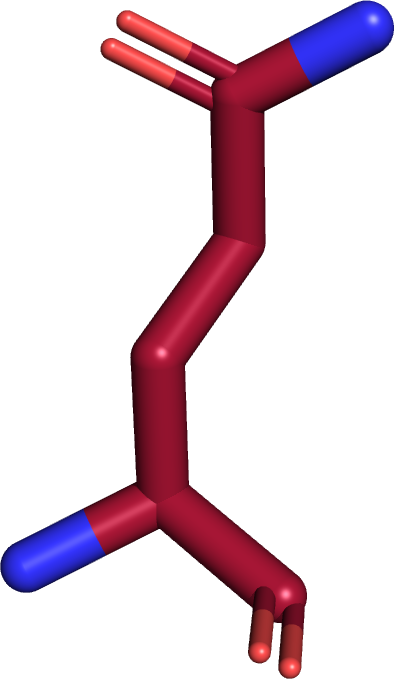
\includegraphics[width=0.25\columnwidth]{bioinfo/figures/amino_acid_Q}};
    \begin{scope}[x={(image.south east)},y={(image.north west)}]
    	\draw[Maroon, thick] (-0.05, -0.05) rectangle (0.85,0.3);
    	\draw[RoyalBlue, thick, dashed] (0.2, 0.35) rectangle (1.05, 1.05);
        %\draw[help lines,xstep=.1,ystep=.1] (0,0) grid (1,1);
        %\foreach \x in {0,1,...,9} { \node [anchor=north] at (\x/10,0) {0.\x}; }
        %\foreach \y in {0,1,...,9} { \node [anchor=east] at (0,\y/10) {0.\y}; }
    \end{scope}
\end{tikzpicture}
} %
\hfil %
\subcaptionbox{Tyrosine (Y) \label{subfig:aminoY}}{\begin{tikzpicture}
    \node[anchor=south west,inner sep=0] (image) at (0,0) {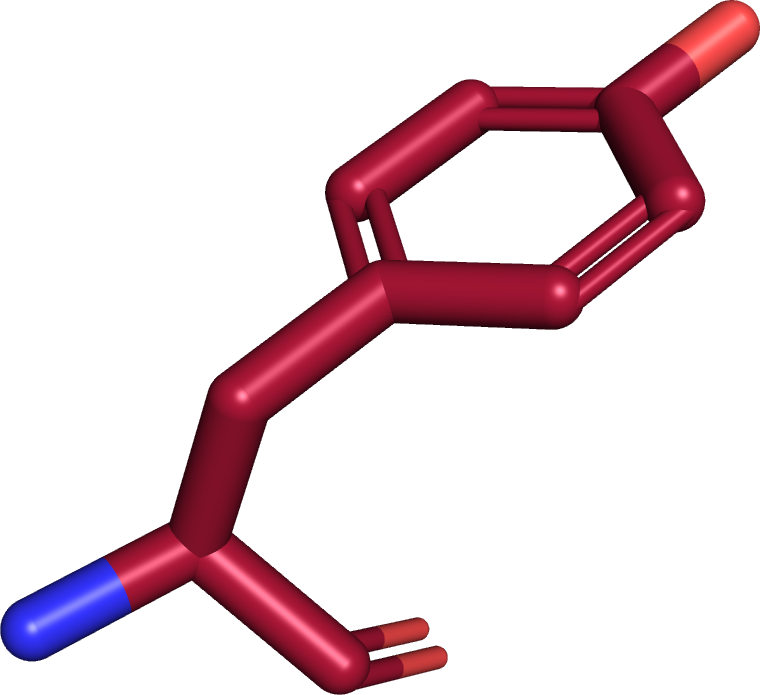
\includegraphics[width=0.45\columnwidth]{bioinfo/figures/amino_acid_Y}};
    \begin{scope}[x={(image.south east)},y={(image.north west)}]
	    \draw[Maroon, thick] (-0.05, -0.05) rectangle (0.6,0.3);
 	    \draw[RoyalBlue, thick, dashed] (0.2, 0.35) rectangle (1.05, 1.05);
        %\draw[help lines,xstep=.1,ystep=.1] (0,0) grid (1,1);
        %\foreach \x in {0,1,...,9} { \node [anchor=north] at (\x/10,0) {0.\x}; }
        %\foreach \y in {0,1,...,9} { \node [anchor=east] at (0,\y/10) {0.\y}; }
    \end{scope}
\end{tikzpicture}
} %
\hfil %
\caption{Two amino acids as appear in proteins.
The \textcolor{Maroon}{maroon}, solid rectangle indicates the backbone, common to all amino acids; and the \textcolor{RoyalBlue}{blue} dashed the side chain, that determines the specific chemical properties.}\label{fig:amino_acids}
\end{figure}

\subsection{Primary structure or sequence}
The amino acids can connect to each other through the peptide bond, forming a chain.
The \emph{primary structure} is the sequence of amino acids as encoded in the \DNA:
\begin{center}
\texttt{ALA ARG ILE ASN GLY ARG GLU ILE ASN VAL THR LYS LYS}
\end{center}

%\missingfigure{peptide bond}

This is the easiest to obtain experimentally since the advent of next-generation sequencing techniques.
These experiments read the \DNA{} of the organism, that can be translated into proteins.
The collection of all protein sequences of an organism is the \emph{proteome}.


\subsection{Secondary structure}
The polypeptide chains are locally organised in motifs stabilised by hydrogen bonds.
The most common is the $\alpha$-helix, \marginpar{$\alpha$} shown in Figure~\ref{subfig:alpha}, where the hydrogen bonds are formed between the backbone oxygen of one residue, and the hydrogen of the amine group, four residues beyond, and continued in a regular pattern, forcing the backbone to twist into a helix.
The same bond is possible with residues that are closer -- two or three -- or further  -- five residues, the $\pi$ helix -- but are less common.

The second most common arrangement is the $\beta$-sheet  \marginpar{$\beta$} depicted in Figure~\ref{subfig:beta}, where approximately extended chains are placed next to each other and bonds are formed between juxtaposed residues.


\begin{figure}[htbp]
	\centering
	\subcaptionbox{$\alpha$-helix\label{subfig:alpha}}{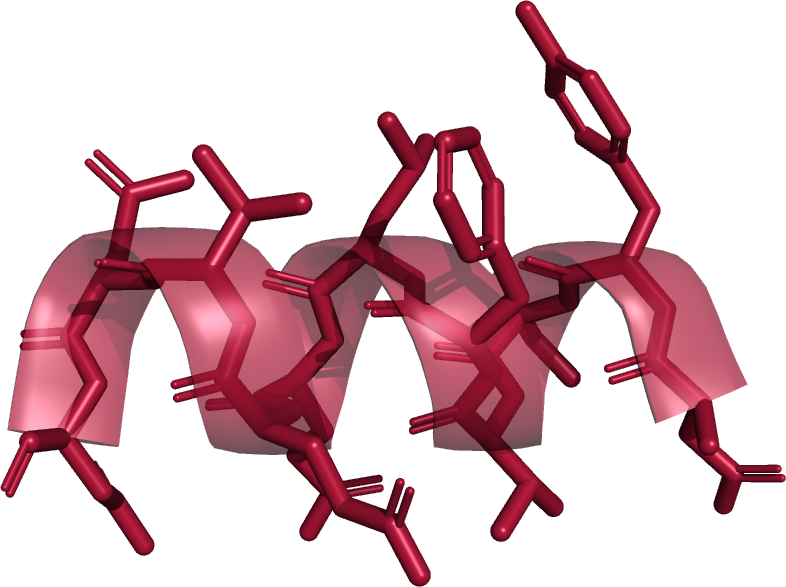
\includegraphics[width=0.9\textwidth]{bioinfo/figures/helix}}\\
	\subcaptionbox{$\beta$-sheet\label{subfig:beta}}{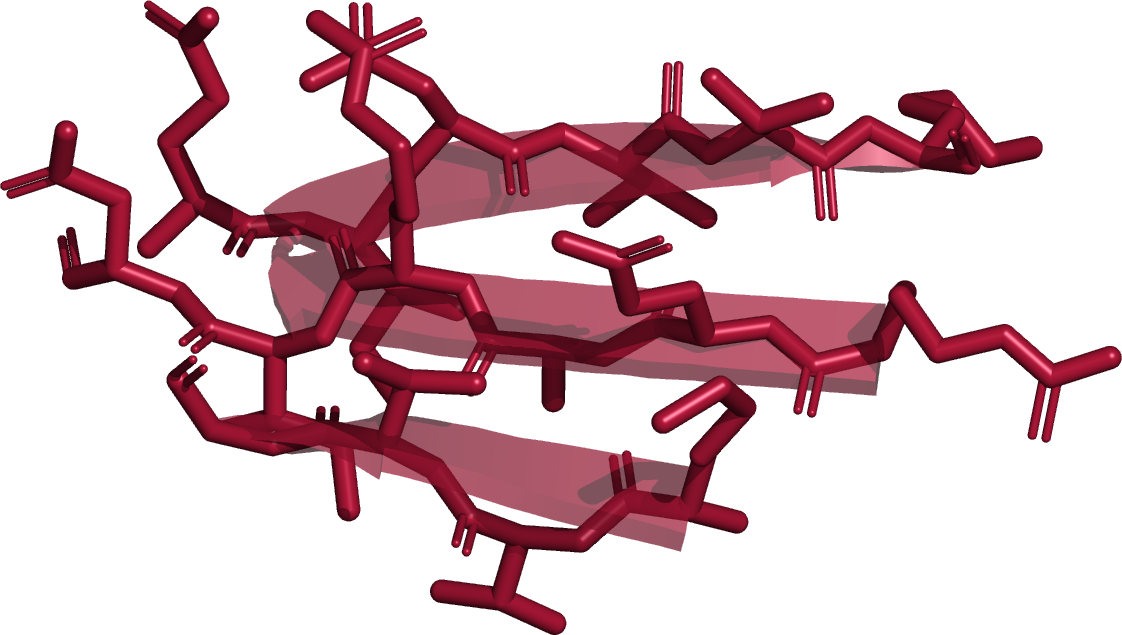
\includegraphics[width=0.9\textwidth]{bioinfo/figures/beta}}
	\caption{The two most frequent secondary structure elements.}\label{fig:alpha_beta}
\end{figure}


\subsection{Tertiary structure}
Once the chain is locally stabilised by the hydrogen bonds it folds into a compact structure.
The spatial arrangement of the secondary structure elements is the \emph{tertiary structure.}
One example is the chain A of the protein \texttt{4V0B}, in Figure~\ref{fig:tertiary}.

\begin{figure}[htb]
\centering
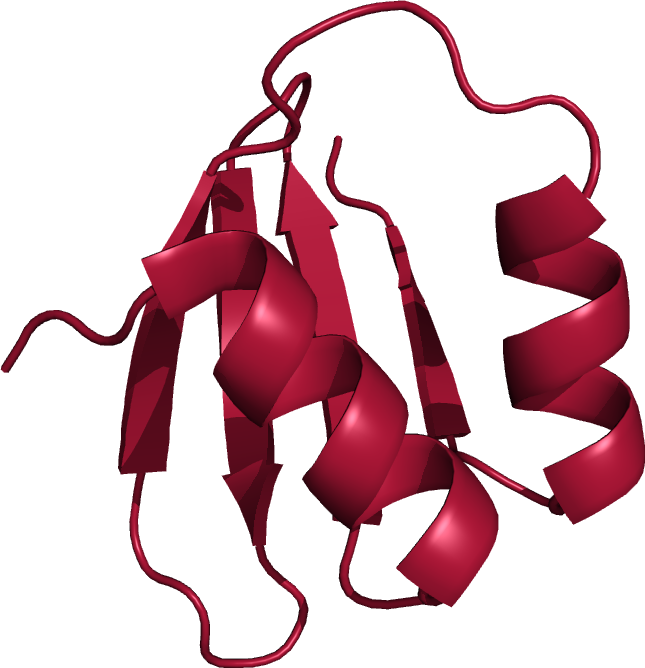
\includegraphics[width=0.8\textwidth]{bioinfo/figures/tertiary}
\caption{The tertiary structure of chain B of the protein \texttt{4V0B}.}\label{fig:tertiary}
\end{figure}

\subsection{Quaternary structure}
Proteins do not always work alone, but they form complexes composed of several chains.
The relative arrangement of each chain is the quaternary structure.

\begin{figure}[htb]
\centering
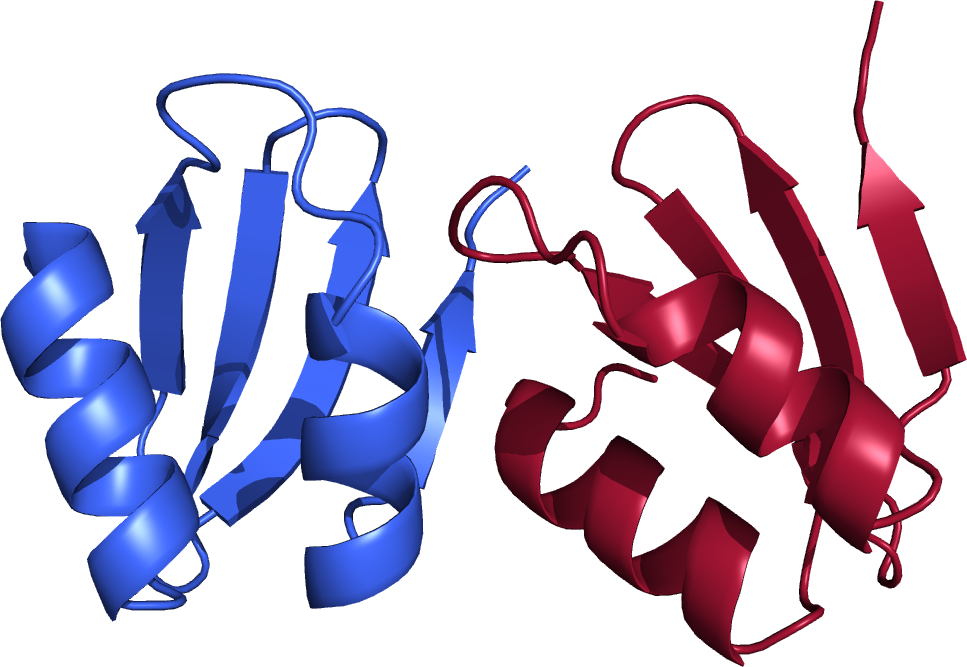
\includegraphics[width=0.8\textwidth]{bioinfo/figures/quaternary}
\caption{Quaternary structure of the chains A and B of the protein \texttt{4V0B}.}\label{fig:quaternary}
\end{figure}

%\subsection{Quintenary structure} %?
\section{Protein biochemistry}

Experiments by \citet{fold_graciously} show that proteins placed in the right medium of pH and temperature will unfold into a random coil, with no trace of tertiary nor secondary structure.
When restored to physiological conditions, they will refold into its natural shape, recovering its original biological and chemical properties.
As long as the protein is chemically unaltered, it will recover the tertiary structure independently of the folding machinery of the cell.
\marginpar{Dogmas that govern protein folding}
This was codified as Anfinsen's dogma: under physiological conditions, the primary structure of globular proteins determines the secondary and tertiary structures, and thus, its function, independently of the cell's machinery \citep{Anfinsen_dogma}.
Typically, the fully folded state is reached in the order of milliseconds to seconds.
The hypothesis has a few exceptions, namely: fibrous proteins, prions -- which are proteins that have an alternative but non-functional stable tertiary structure\footnote{Infamous cause of the mad cows disease.} --  aggregating proteins -- where the individual proteins bind to each other forming large and non-functional structures\footnote{For example, the cause of Alzheimer and Multiple Sclerosis} -- and large, multi-domain proteins.
A reasonable hypothesis is that a priori, the native conformation seems to be the state in the lowest energy, and the random coil is just rolling down the energy landscape.

Cyrus Levinthal \marginpar{Levinthal's paradox} noted that, for every amino acid, a protein has two main degrees of freedom corresponding to the torsion of the backbone, plus one more for the rotation of the side chain.
This gives us a configuration space of the order of $10^{2L}$ for a protein of $L$ residues, but the kinematics suggest that it only has time to sample $10^8$ conformations, an exponentially tiny fraction for proteins of typical length.

Levinthal suggested two corrections:
\begin{itemize}
	\item The native conformation is not necessarily the one of minimum energy, but a local meta-stable minimum with a deep enough well that it is stable.
	For most proteins, this is not very deep, around 10-\SI{15}{\kilo cal/\mol}.
	\item The native conformation must be kinematically accessible, possibly guided by local interactions that partially fold the protein.
	In other words, the energy landscape of protein folding presents a wide funnel from the unfolded state to its near-native conformation, which allows for a rapid transition.
\end{itemize}

%These corrections are supported by experiments showing that a certain enzyme only folds at temperatures around 37 C, but it is completely stable up to 90 C.
%Furthermore, the same enzyme produced by an organism that lives at colder temperatures is shown to require lower temperatures for renaturation, but it is still stable up to 90 C.
%The order of events greatly influences the kinetics of folding.

%\FloatBarrier
%\subsection{The protein backbone}
\subsection{The hydrophobic effect}
Water molecules are electric dipoles with a partial negative charge on the oxygen, and a partial positive charge on the hydrogens.
This introduces an electrostatic interaction between molecules in bulk of water, that self-organises to form a network of hydrogen bonds.
Any non-polar molecule submerged in water will disrupt this network of bonds.
To preserve as many energy-favourable hydrogen bonds the water molecules near the boundary can reorient themselves, forming a pocket around the hydrophobic substance in the process.
The degrees of freedom for the boundary is restricted, so the entropy -- and consequently the free energy -- is reduced.
This is the \emph{hydrophobic effect}, responsible for the immiscibility of fats and water.

A protein chain \marginpar{Hydrophobicity and folding} \todo{This is weird? H-network}
will be composed of both hydrophobic and hydrophilic amino acids.
When placed, unfolded, in the cellular environment, tiny pockets of water will be created around the hydrophobic regions.
Quickly, these pockets will join together, expelling most of the water and forming a compact core of hydrophobic residues, surrounded by hydrophilic ones, the \emph{molten globule}.
A partial secondary structure, close to native, is observed.

\subsection{From molten globule to structure}
The core of the molten globule is not completely devoid of solvent, which slightly increases the distance between adjacent elements, greatly reducing the van der Waals interactions.
Long-range contacts are not preserved, which indicates a relative flexibility between its components.
Our globule is ``soft" and ``wet".

The transition to the solid, native state, involves the repacking of the side chains into a tight and compact core.
This process finalises the packing of secondary structure and freezes most of the long-range contacts.

It is noteworthy \marginpar{Further discussion}
that not all proteins present a molten globule, and can transition directly between coil and native \citep{protein_physics}.


\subsection{Energy terms}
A relatively generic form of the energy dictating the dynamics of a protein is:
\begin{align*}
H(\left\{\vec r_i\right\}_{i=0}^N) =& \underbrace{\sum_{bonds} k_b \left(d - d_0\right)^2}_\alpha + 
\underbrace{\sum_{angles} k_a \left(\theta - \theta_0\right)}_\beta +  \nonumber \\
&+ \underbrace{\sum_{torsions} f\left(\omega\right)}_\gamma +
\underbrace{\sum_{free\ pairs} k_{ij} \left[\left(\frac{r_{0ij}}{r_{ij}}\right)^{12} - 2 \left(\frac{r_{0ij}}{r_{ij}}\right)^{6} \right]}_\delta + \nonumber \\
&+ \underbrace{\sum_{i,j} \frac{q_i q_j}{4 \pi \epsilon r_{ij}}}_\epsilon
\end{align*}
The terms correspond to:

\begin{itemize}
\item[$\alpha$] A harmonic potential on the bond lengths $d$ for every pair of covalently bonded atoms, where $d_0$ is the ideal bond length and $k_b$ is the strength of the potential for the atom types.
\item[$\beta$] A harmonic potential on the angles between adjacent bonds $\theta$.
\item[$\gamma$] An arbitrary function $f$ on every torsion angle $\omega$.
\item[$\delta$] The Lennard-Jones potential between all pairs of atoms not covalent bonded, where $r_{0ij}$ denotes the equilibrium distance and $k_{ij}$ the depth of the energy well.
This term corresponds to the van der Waals forces.
\item[$\epsilon$] The electrostatic energy between charges, assuming they are spherically distributed.
\end{itemize}

Note that the collection $\vec r_i$ % $\left\{\vec r_i\right\}_{i=0}^N$
includes the water molecules and other atoms in the environment of the protein itself.

Of these terms, $\alpha$ and $\beta$ are strictly valid only near their respective minima, while $\delta$ is valid for distances around and beyond the minimum.
In practice, this is not a significant problem because the deviations from the ideal values are small. \marginpar{Dynamics}
From here we can see that most of the dynamics in proteins is given by the flexibility of the torsion angles.
Roughly speaking the torsions of the backbone determine the secondary structure and those of the side chains, the packing.

\todo{Entropic terms}

%\section{Membrane proteins}
%\todo{membrane proteins}
\section{Experimental methods}
How can we know the structure of a protein?
The most commonly used methods are X-ray crystallography and \NMR{} spectroscopy.


X-ray crystallography starts by
\marginpar{X-ray}
purifying and crystallising the protein, and observing the diffraction pattern of an X-ray beam.
The X-rays interact with the protein, diffract, and form a pattern of dots that is proportional to the intensity of the Fourier transform of the electron density.
By taking the inverse transformation, the crystallographers can reconstruct the electron density, and then fit an atomic model.
The X-ray detector -- a photographic plate or a \CCD{} sensor -- can only measure intensities, not phase information.
Experimentalists have to apply an iterative process where they combine estimated phases from models with the real intensities.

One criticism of X-ray crystallography is that the proteins are in crystals, not in physiological conditions.
The alternative method is Nuclear Magnetic Resonance (\NMR) \citep{nmr}, \marginpar{\NMR} which applies strong oscillating magnetic fields and measures resonances.
From the spectrum, one can identify distances between atoms with non-zero nuclear spin.
The method cannot provide sufficient constraints to determine the whole system, so it is given as an ensemble of models instead.
The differences between individual structures can be caused by natural movements of the protein, or by uncertainties in the experiment itself.

In the last decades, \marginpar{cryo-\EM}
a new method has become practical for protein structures: cryogenic electron microscopy.
In this method, the protein samples are placed in solution on a thin sheet of solution, flash-frozen to cryogenic temperatures, and put under an electron microscope.
Since proteins are diluted, each one is frozen in a random orientation, so each image is a \textsc{2d} projection along a different axis.
The various images are clustered and combined to reduce noise, and a \textsc{3d} model is inferred from it.

This technique allows us to study large complexes in solution, without the necessity to crystallise them.
It can reveal the presence of unknown proteins, and even provide information on the thermodynamics:
The Boltzmann distribution says that the probability of a state $x$ depends on the energy of the system:

\begin{equation*}
p(x) \propto e^{-\frac{H(x)}{k_B T}}
\end{equation*}

So, when we have a sample with different conformations of the same protein, counting the number of images that correspond to each state gives us a measure of the difference of energies between the two states.

The development of Cryo-EM was recognised in 2017 with the award of the Nobel Prize in Chemistry \emph{"for developing cryo-electron microscopy for the high-resolution structure determination of biomolecules in solution"} to Jacques Dubochet, Joachim Frank, and Richard Henderson  \citep{cryoEM_nobel}.


\subsection{Partial restraints}
Sometimes, an experiment to obtain the full structure is not possible.
There are simplified methods that, while they cannot give a full structure, they may be able to provide enough constraints for computational methods.

The first is Small Angle X-ray Scattering, or \SAXS. \marginpar{\SAXS}
The process is similar to X-ray crystallography, but now the protein is in solution.
Each unit will produce its own interference pattern, but since they are not crystallised, the orientation of each pattern is randomised.
From this we can infer a rough shape of the protein, and the presence or absence of differences between conformations.

A related method is Small Angle Neutron Scattering, or \SANS. \marginpar{\SANS}
It replaces X-rays with neutrons, which changes the sensitivity to different nuclear species.
In particular, hydrogen has one of the largest cross-sections.
One application is the study of membrane proteins in an appropriately chosen detergent, which can be almost invisible to the neutron beam.
More information on both methods can be found in the work of~\citet{sax}

Mass-spectrometry cross-linking \citep{cross_linking} \marginpar{Cross-linking} can be used to measure distances within proteins.
The protein is mixed with a reagent that connects to specific functional groups of amino acid side chains.
Then, an enzyme is added that cleaves the protein, and the fragments are sent to a liquid chromatography tandem mass spectrometer that analyses the composition of each fragment.
The linkers keep the fragments split by the digestion together, from which we can infer they were in contact.
Furthermore, since we know the size of the linker, we can have an accurate upper bound on the distance.


\chapter{The informatics of biology}
Bioinformatics is the application of computational methods to biological problems,
either by analysing large amounts of data or by replacing experiments with computer programs.

\section{Predictors}
A significant fraction of the protein bioinformatics work is the development of predictors: statistical or machine learning methods that can, given limited information, predict properties of proteins.
A common choice is to make predictions taking only the amino acid sequence because this is the easiest information we can acquire of a protein.
Other methods may require extra annotation, such as Gene Ontology -- an annotation condensing all our knowledge of the gene that produced the protein -- or 3D structures -- experimental or models.

\section[Multiple Sequence Alignments]{Increasing statistics: Multiple Sequence Alignments}
Proteins, as well as organisms, are products of evolution.
, so we can find similar versions of the same protein in different organisms.\todo{introduce evolution}
Even when the function is novel, it usually evolves as a minor modification of pre-existing proteins.
This means that, in most cases, we can obtain a better prediction when working at the \emph{family level,}
i.e., considering not only our protein of interest but also any related sequence in our database.

To have coherent statistics, every sequence must be aligned to the original query, as in the following example:

\begin{center}
\marginpar{\phantom{a}}
\marginpar{\phantom{a}}
\marginpar{\phantom{a}}
\marginpar{An example \MSA}
\begin{Verbatim}[fontsize=\small, xleftmargin=1em]
1       10        20        30        40        50   
FCLEPPYTGPCKARMIRYFYNARSGSCETFIYGGCKAKRNNFKSEEDCMRTCG
FCREPPYTGPCSAHFVRYFYNATTGLCQSFVYGGCRGKQNNFMDEKECLHTCD
FCREPPYTGPCRAHFIRYFYNATTGLCQTFVYGGCRGKQNNFMDEKECLHTCD
ICSMKNDTGPCKAYMPRWFFNSQTKQCEEFIYGGCSGNNNNFMTREDCCNSCS
-CTLPKVPGPCNAYFVRWWYDQQKEICSSFIYGGCQGNNNNFQSESVC-----
------DPGPCKAYMPRFYFEIEKKECQEFIYGGCGGNENRFFTKRECQRICK
ECLMAPDPGNCGGVRERWFFSPEAKQCRLFGYSGCQGNANNFATIEDCMAKC-
LCHLAMESGPCRAAKPRWYFDQGKQTCVEYIYGGCRGNSNNFETKAECMRTCS
-CEQAMDPGPCKAAFPRWYFNSQTGQCEQFIYGGCLGNDNNFVTEQECQTTCG
\end{Verbatim}
\end{center}

The collection of sequences is called a Multiple Sequence Alignment, or \MSA.
Here, the dash \texttt{-} indicates a gap, a residue that is not present at that particular position.
This section explains how to build it.


\subsection{Pairwise alignment}
The building block of an \MSA{} is the alignment of each related sequence to our query, and the first step is to measure how similar they are.
The most basic scheme simply counts the number of matching amino acids, assigning a positive score for matches, and a penalty for mismatches.

Proteins \marginpar{The reason for gaps} have insertions and deletions, which means the matching regions in different proteins may be discontinuous.
We can allow for gaps in the scores including a term that considers both opening -- our belief of how common insertions and deletions are -- and extending the gap -- considering our expectation of their length.

Furthermore, not all mismatches are the same.
For example, leucine (L) and isoleucine (I) are functionally very similar, and can often be replaced without loss of function.
On the other hand, a single mutation from glutamic acid (E) to valine (V), in humans is enough to cause sickle cell anaemia.

Nor are all matches.
Alanine (A) forms over $7\%$ of the proteome, so we are more likely to find a hit at random than with tryptophan (W), which forms less than $2\%$.

We can codify \marginpar{Substitution matrix} the difference between different amino acids in a substitution matrix.
The most common choice to detect distantly related proteins is the \textsc{blosum} family.
\citet{blosum} derived them from a set of 500 multiple sequence alignments.

\subsection{Scaling up: \BLAST}
Performing a pairwise alignment on a large sequence database would be very slow, but for a given query, most entries in the database are not related.
Programs like \BLAST{} (Basic Local Alignment Search Tool, \citep{blast}) introduce a set of heuristics to discard negatives as quickly as possible.
They do not guarantee an optimal alignment according to the scoring matrix, but they compensate it by being able to produce a much higher amount of data.

\subsection[\PSSMs and  \PSIBLAST]{Position Specific Scoring Matrices and \textsc{psi-blast}}

Substitution matrices assume a fixed evolution model, and that every residue is as important as every other.
But this is not true, we can observe that some protein regions are highly conserved because they are, in one way or another, important for the function of the protein.
In the earlier example, we can see how around column 40, there are fewer changes.
We want our search to reflect this fact, and, for instance, only accept changes in these regions if they provide enough similarity in the rest of the protein to support the fact that they are related.

\PSIBLAST{} \citep{psiblast} does this using an iterated search, and building Position Specific Scoring Matrices (\PSSM).
The first iteration is a normal \BLAST{} search, using the default substitution matrix, but in the subsequent iterations, it uses the statistics of each column to update the substitution matrix.
Since each position is treated independently, it can model better the importance of each residue.

\subsection[Hidden Markov Models]{Increasing sensitivity with Hidden Markov Models}
\PSSMs{} can model the differences in probabilities for each amino acid at different positions, but gaps are still modelled with a flat penalty across the sequence.
We know this is not a good representation of proteins, since they are unlikely to happen in the core due to the lack of space.
Insertions are easy to introduce in short, external loops; and deletions are most likely in long loops. 
A representation that allows us to model both mutations and insertions and deletions with different rates at different positions are Hidden Markov Models (\HMM).

An \HMM{} \marginpar{The \HMM} is a probabilistic model, where the system travels across a series of hidden states following a Markov chain, a model with discrete states where the probability of transition depends only on the current state -- ignoring the history.
We do not have access to these states -- hence \emph{hidden}.
Instead, each of them has a certain probability of emitting a symbol: the observed amino acids.
Fitting a Hidden Markov Model consists on figuring the emission probability for each state -- the analogue to the \PSSMs{} -- and the transition probability between states.
Like in \PSIBLAST, this is done iteratively, passing several times through the data and updating our belief.

The two most popular programs to perform these searches are \JackHMMER \citep{jh}, and \HHBlits \citep{hhblits}:

\begin{itemize}
\item \JackHMMER{} compares every sequence in the database with its \HMM.
It performs an \HMM-sequence comparison.
\item \HHBlits{} uses a database of pre-computed \HMMs{} based on sequence clusters.
It compares \HMM{} to \HMM, and in case of a match, includes all the members of the cluster in the \MSA.
\end{itemize}

\JackHMMER is slower
\marginpar{Advantages and disadvantages}
because it must consider each sequence; but it can search against any database without the need to pre-prepare it.
\JackHMMER can easily keep an up-to-date sequence database, or work on databases tailored for the search at hand.

On the other hand, each \HHBlits{} search is faster since it only needs to compare once against each cluster, but it requires a lot of computational resources to perform the initial clustering.
This means the databases are not updated as often, and only a handful of versions are available.
Furthermore, since all the members of each cluster are added, the \MSA{} has sharp boundaries at the edges of each one.



\section[Protein structure prediction]{\emph{In-silico folding:} Protein structure prediction}
One of the main goals of protein bioinformatics is predicting the 3D structure of a protein given only its sequence.
In this section, I will present the main strategies.

\subsection{Physics-based modelling}
Unfolded natural proteins in physiological conditions are known to fold into their native state \citep{fold_graciously}.
In principle, the same procedure can be replicated \emph{in silico} with molecular dynamics, like the work done by \citet{physics_folding}.
This was possible because the domain is very short -- 35 residues -- and fast folding; but in general is not a practical solution, as it requires a lot of computational work.

\subsection{Homology modelling}
Proteins that are close in sequence are close in structure, so if we can find a protein of known structure that has a sequence close to our protein of interest, we can use it as a \emph{template}.
When a good hit is found, this is the most accurate and reliable modelling strategy.

\MODELLER~\citep{modeller}, for example, uses the templates to infer distance restraints, uses geometrical algorithms to create an initial model, and then relaxes it with a short molecular dynamics run.


\subsection{\emph{Ab-initio} folding}
In the absence of available templates, we can use \emph{ab-initio} or \emph{template-free} methods, in which we try to find the minimum energy of the system, including additional terms derived from predictors.

Rosetta's \citep{Rosetta3} \marginpar{Rosetta} \emph{ab initio} protocol implements a simulated annealing scheme that starts with an extended chain and randomly replaces fragments with ones derived from the \PDB.
Since the fragments are taken from real proteins, the models tend to have good chemical properties, even when completely wrong.
In order to speed up and improve convergence, we can add additional energy terms to the force field, such as contact restraints.

\CONFOLD~\citep{confold} \marginpar{\CONFOLD} is the other protocol used in this thesis.
It is build upon \CNS, and works by transforming contacts and secondary structure to a large set of distance restraints between atoms.
Then, it runs a geometric solver, followed by a fast relaxation.
This method is much faster than Rosetta, but since it lacks the chemical information of the fragments, it does not work well on regions without contacts.


\subsection{Evaluation}
Once we have a model, how can we compare it with the native structure? How can we measure how accurate it is?

One option is to superimpose model 
\marginpar{Superposition}
in such a way that the metric is optimised.
Given two structures with $L$ residues in common, and being $d_i$ the distance between the $i-$th residues of both structures, we define the distances as:

\RMSD, or the Root Mean Squared Deviation:
\begin{equation*}
\RMSD = \min \left(\sqrt{\frac{\sum_{i=1}^L d_i^2}{L}}\right),
\end{equation*}

The \Ss-score (Superposition score) is:
\begin{equation*}
S = \max\left[\frac{1}{L} \sum_{i=1}^L \frac{1}{1 + \left(\frac{d_i}{d_0}\right)^2}\right],
\end{equation*}
where $d_0$ is a parameter to be decided, usually $\SI{3}{\angstrom}$.

The \TM{} (Template Modelling score) is the same as \Ss, but $d_0 = 1.24 \sqrt[3]{L - 15} - 1.8$, to keep TM roughly independent of the length.

Both \Ss{} and \TM{} scores give values between $0$ and $1$.
For TM, values below $0.3$ correspond to random structures, and scores over $0.5$ indicate structures about in the same fold \citep{tmscore05}.

The problem with superposition scores is that are sensitive to conformational changes.
For example, consider a protein composed of two subunits connected by a small, flexible hinge; and a model where each of the subunits is perfect, but the relative orientation is not the same.
The superposition scores would align one of the subunits, with perfect scoring, and give bad values to the other.

A solution is to compare structures locally. 
\LDDT{} (Local Distance Difference Test) \citep{lddt} \marginpar{\LDDT}
measures, for every atom, the fraction of preserved  distances, up to a given tolerance, within an inclusion radius.
\LDDT{} considers all inter-atomic distances that are within $\SI{0.5}{\angstrom}$, $\SI{1}{\angstrom}$, $\SI{2}{\angstrom}$, and $\SI{4}{\angstrom}$.
The final scores is obtained averaging over all the atoms in the residue and inclusion thresholds.

\citet{cad} proposed a similar method, using surface contacts instead of distances. \marginpar{\CAD}
They represent each residue as the Voronoi volume of its atoms.
The surface area for the contact between residues $i$ and $j$ of the model is $S_m(i,j)$, and for the reference -- native structure -- $S_r(i,j)$.
\CAD{} score is proportional to the difference between the two, with some normalisation terms:

\begin{equation*}
\CAD_{score} = 1 - \frac{\sum_{i,j} \min\left( \left| \: S_{r}(i, j) - S_{m}(i, j)\right|, S_{r}(i, j)\right)}{\sum_{i,j} S_{r}(i, j)}
\end{equation*}

\subsection[Model Quality Assessment]{Model Quality Assessment, or Estimation of Model Accuracy}
The previous section dealt with the case where we know the native structure, but what can we do when we do not know it?
After all, if we have the experimental data, there is no need for modelling.
The task of predicting the quality of a model is called \emph{Model Quality Assessment} (\MQA), or in some modern papers, \emph{Estimation of Model Accuracy} (\EMA).
The purpose of \MQA{} is two-fold:

\begin{itemize}
\item \emph{Model selection}, or picking the best model from an ensemble generated by one or different methods.
\item \emph{Model evaluation}, or estimating the overall quality, or how much it can be trusted.
Some applications may require high-quality models, while for others, knowing the right fold is sufficient.
\end{itemize}

In principle, \marginpar{Energy-based \MQA?} we could compute the energy of each model, assuming that the lower the energy, the closer we are to our target.
This has two flaws: it does not provide information about \emph{how far} -- since in principle we do not know the energy of the native state -- and it is not a reliable way of comparing models from different methods -- because energy functions are very sensitive to small details.
Consider the case of a perfect model, except for two atoms that are in the same position.
The scores presented on the previous section would all be close to 1, but the energy would be infinite!

We can partially remediate this problem by repacking the models using a common energy function, but this method would still favour models that were optimised with the same energy function we are using.


The alternative solution is to use machine learning and try to predict scores directly.
\marginpar{Unsupervised: clustering}
We can use unsupervised programs, like Pcons \citep{pcons}, that cluster the models, and select the one that is closer to the centre.
The underlying assumption is that, if several independent methods agree, they are probably correct.
If all our models come from a single method, but the set of restraints is good, they will all be similar; but if the restraints are insufficient or contradictory, the models will be diverse.
They are called \emph{consensus methods}.

The alternative is to use supervised machine learning,
\marginpar{Supervised}
describe the model with a set of features, and try to predict in isolation its quality.
The features we can use fall into two categories:

\begin{itemize}
\item Description of physico-chemical properties, such as energy terms and torsion angles.
\item Agreement with predictors, such as secondary structure. A good model should have a good agreement with predictors, but not necessarily perfect.
\end{itemize}

This approach is called \emph{single method}, and in this thesis, we have developed two supervised single methods (Papers \textcolor{Maroon}{I} and \textcolor{Maroon}{IV}).


\section{Contact prediction}\label{sec:contacts}
To be able to predict a structure without a template, we need an crucial  bit of additional information: the contact map, or the collection of residues that are in contact.
We usually define \emph{contact} \marginpar{Distance threshold} as closer than $\SI{8}{\angstrom}$ between the C-$\beta$ atoms,
but other authors may use $\SI{10}{\angstrom}$ between C-$\alpha$, $\SI{4}{\angstrom}$ between any pair of heavy atoms, or combinations.

Folded proteins \marginpar{How is this possible?} are tightly packed structures, as illustrated in Figure~\ref{fig:packing}.
Since there is very little to no space between neighbouring residues, not every mutation is allowed.
When a protein gains a mutation, it usually needs to be compensated by others somewhere else in the protein to keep it stable.
\marginpar{Correlated mutations}
For example, if an amino acid is replaced by a bigger one, a nearby residue would have to be changed for a smaller one; or if a neutral amino acid gains a positive charge, it would be energetically favourable to have a negatively charged next to it.
Contacts in our protein, or residues nearby in space, will appear as sets of correlated, compensating mutations in an \MSA.

\begin{figure}[!htb]
	\centering
	\hfil
	\subcaptionbox{Cartoon and sticks\label{subfig:sticks}}{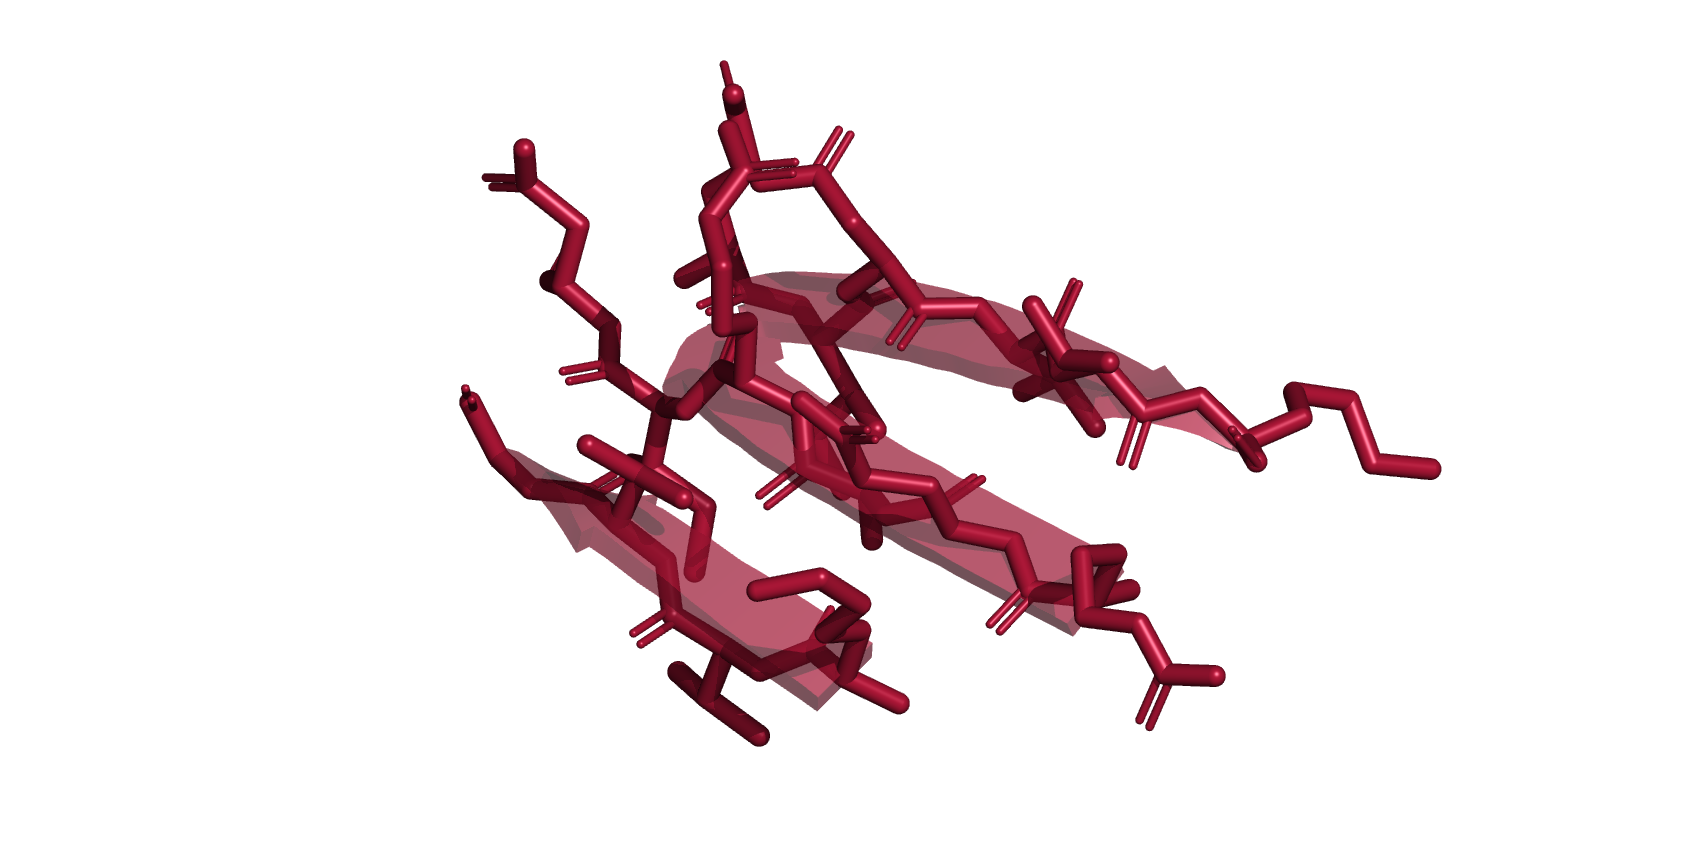
\includegraphics[trim={65mm 3mm 32mm 0},clip, width=0.45\textwidth]{bioinfo/figures/sheet_sticks}}
	\hfil
	\subcaptionbox{Atom-sized spheres\label{subfig:spheres}}{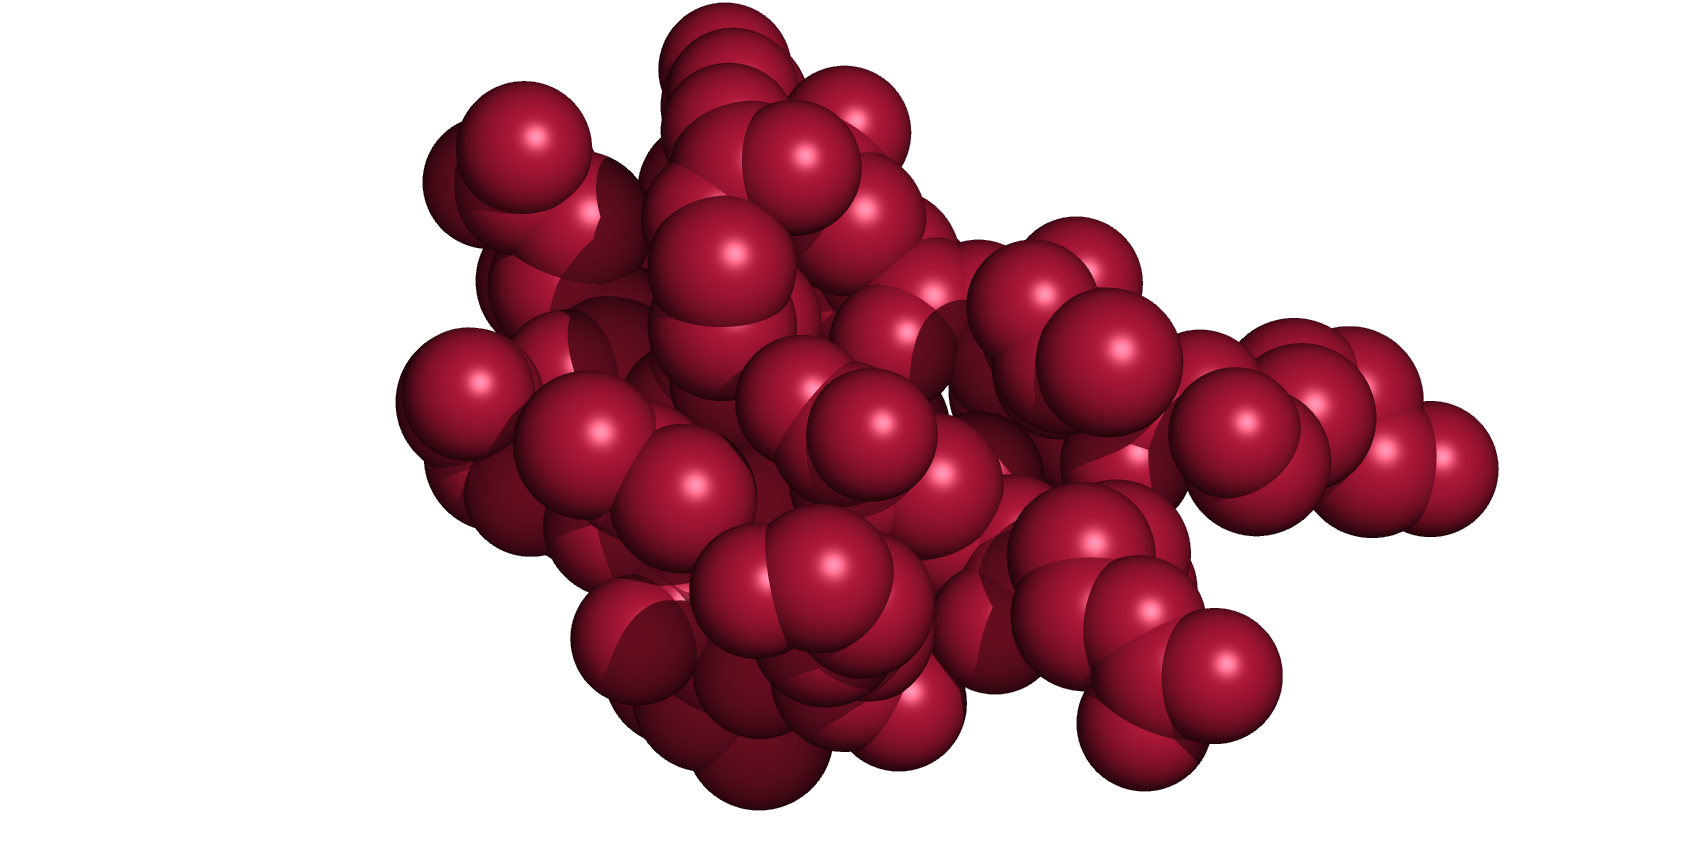
\includegraphics[trim={65mm 3mm 32mm 0},clip, width=0.45\textwidth]{bioinfo/figures/sheet_spheres}}
	\hfil
	\caption{Fragment of a $\beta$-sheet in two representations: cartoon and sticks, and space filling spheres, showing the tightness of the packing.
	They are both seen from the same angle at the same scale.}\label{fig:packing}
\end{figure}


\subsection{Mutual Information}
How can we formalise mathematically correlated mutations?
Mutual Information codifies the information gain that we can obtain for one distribution knowing the other, and considering the relative distributions.
The formula is:

\begin{equation*}
MI\left(i, j\right) = \sum_{x, y}^{q_{max}} f(x_i, y_j) \log \left(\frac{f(x_i, y_j)}{f(x_i)f(y_j)}\right),
\end{equation*}
where $f(x_i, x_j)$ is the joint distribution of amino acids $x_i$ and $y_j$ at positions $i$ and $j$, $f(x_i)$ and $f(y_j)$ are the marginal distributions, and $q_{max}$ is the maximum number of amino acids types in the alignment, including gaps.
Note that if $x$ and $y$ are independent, $f(x_i, y_j) := f(x_i)f(y_j)$, the logarithm vanishes, and thus $M(i, j) = 0$.
If the \MSA{} is of enough quality, the contacts will present high values of $MI$.


\subsection{Direct Coupling Analysis}
Mutual Information has a problem with the transitivity property: consider three residues, A, B, and C; where B is close to both A and C, but A and C are far away.
Mutual Information will likely detect a correlation between A and B, and between B and C; but it will also show a correlation between A and C!

To discern true from spurious correlations, we need to fit a statistical model to the whole data at once, in this way, we hope to recover the true (direct) relationships.
This can be accomplished with Direct Coupling Analysis (\DCA).
Several variations exist, but they are all based on a Potts model of statistical mechanics.
This is a model where each position (in our case, residue), can take a number of discrete, well-defined, spin states (amino acid types), and the model depends only on the intrinsic properties at each location, and pairwise interactions.

The energy of a sequence of amino acids $\vec{\sigma}$ takes the form:
\begin{equation*}
H(\vec \sigma) = \sum_{\substack{i,j=1\\i \neq j}}^N J_{i, j}(\sigma_i, \sigma_j) + \sum_{i=1}^N h_i(\sigma_i),
\end{equation*}
where $h_i(\sigma_i)$ is the chemical potential of having a given amino acid at position $i$, and $ J_{i, j}(\sigma_i, \sigma_j)$ is the pairwise interaction between residues $i$ and $j$ given their amino acid species.

We can assume the proteins in our \MSA{} were generated by a similar model, so their frequency should follow the Boltzmann distribution:

\begin{equation*}
p(\vec{\sigma} |  h, J) = \frac{1}{Z} e^{-\beta H\left(\vec{\sigma}\right)}
\end{equation*}
$\beta$ is a scaling factor, the inverse of the temperature, and $Z$ is the partition function, a normalisation term to ensure all the probabilities sum up to 1:

\begin{equation*}
Z = \sum_{\vec{\sigma}} e^{-\beta H\left(\vec{\sigma}\right)}
\end{equation*}

Fitting a Potts model means to estimate the values of $J$ and $h$ that best explain the observed distribution of sequences in the \MSA.
The problem as such is intractable because computing $Z$ implies a sum over all the possible sequences of length $N$, $21^N$ (the 20 natural amino acids plus the gap state).

Several strategies can approximate the partition function, such as \plmDCA~\citep{plmDCA}, or side-step it all together, like \GaussDCA~\citep{GaussDCA}.

Once the values of $J$ are obtained, the scores of the contacts can be estimated by taking the Frobenius norm of each of the J matrices.
That is, the square root of the sum of the squares of the couplings between each pair of amino acids:

\begin{equation*}
C(i, j) = \sqrt{\sum_{\sigma_i, \sigma_j=1}^{21} J_{i, j}(\sigma_i, \sigma_j)^2},
\end{equation*}
where $C(i, j)$ is the contact score between residues $i$ and $j$.
This number cannot be readily interpreted as a probability.

This model approximations ignore the possibility of multiple rotamers for a given amino acid \marginpar{The sphericity of the cow}
and consider that any interaction between three or more residues can be decomposed to the sum of each pair.
Finally, \DCA{} attempts to reconstruct the evolutionary couplings, not necessarily the contacts.
\citet{contact_errors} showed that most of the top-scoring pairs indicated by \DCA{} are true contacts, others correspond to contacts between different subunits in a homodimer or pairs of separated residues involved in the function.
The coupling is real, but its nature is different from the model explained at the beginning of this section.

\subsection[Phylogenetic bias]{Phylogenetic bias: the \APC{} correction}
Natural proteins are not randomly drawn from a generative model, like Potts.
Proteins evolve alongside a tree, where a mutation in an organism is likely to be shared among all the descendants.
This appears as a pattern of vertical and horizontal lines on the contact map, as seen on the upper triangle of Figure~\ref{fig:apc}.

\citet{apc} proposed a simple method to reduce this bias: for each column in the contact map, subtract the average of the row times the average of the column, normalised by the total average.


\begin{figure}[hbt]
	\centering
	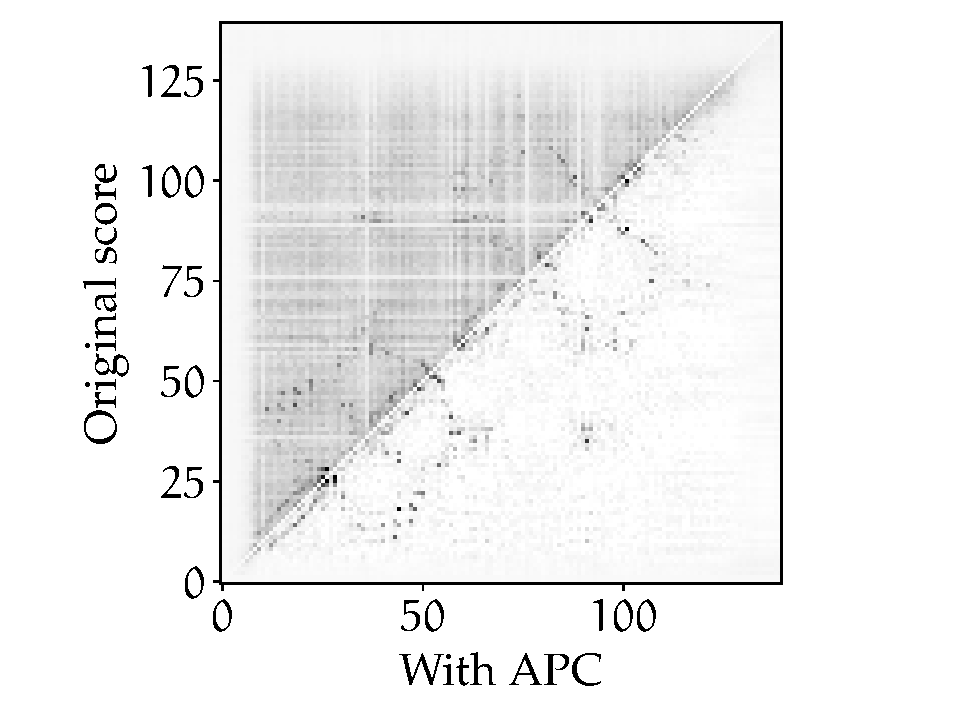
\includegraphics[trim={12mm 3mm 26mm 3mm},clip,width=0.7\textwidth]{bioinfo/figures/apc}
	\caption{Contact scores without (upper) and with (lower) the \APC{} correction.
	The patterns are clearer in the lower triangle, and most of the bias shown as vertical and horizontal stripes has been removed.}\label{fig:apc}
\end{figure}


\subsection{Pattern recognition}
Contacts do not appear at random.
Since the protein is a continuous chain, contacts are rarely isolated, and appear in groups.
Furthermore, since most of the protein is locally organised in secondary structure elements, this gives rise to specific patterns in the contact map, as can be seen in Figure~\ref{fig:contact_patterns}.
The statistical methods like \DCA{} and Mutual Information do not consider this, so a refinement step can be done using pattern recognition.
We can train a machine learning algorithm on the outputs of statistical methods and recognise the underlying patterns, which can remove much of the spurious contacts, noise, and artefacts in the alignments.

This was the focus of our contributions on Paper \textcolor{Maroon}{IV}.

\begin{figure}[!htb]
	\centering
	\hfil
	\subcaptionbox{Alpha helices, with their characteristic chequerboard pattern.\label{subfig:alphacontact}}{\begin{tikzpicture}
    \node[anchor=south west, inner sep=0] (cmap) at (0,0) {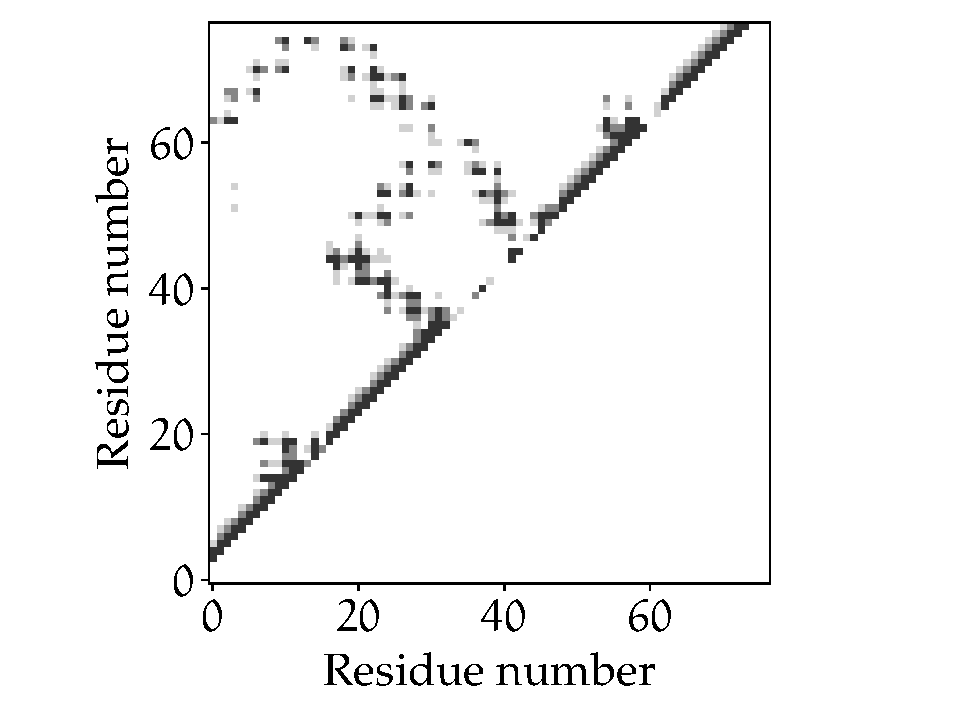
\includegraphics[width=0.45\columnwidth]{bioinfo/figures/alpha_contactmap_base}};
    \node[anchor=south west, inner sep=0] (prot) at (2.5,0.9) {\includegraphics[width=0.13\columnwidth]{bioinfo/figures/alpha_prot}};
\end{tikzpicture}
}
	\hfil
	\subcaptionbox{Beta strands, showing the typical parallel bands\label{subfig:betacontacts}}{\begin{tikzpicture}
    \node[anchor=south west, inner sep=0] (cmap) at (0,0) {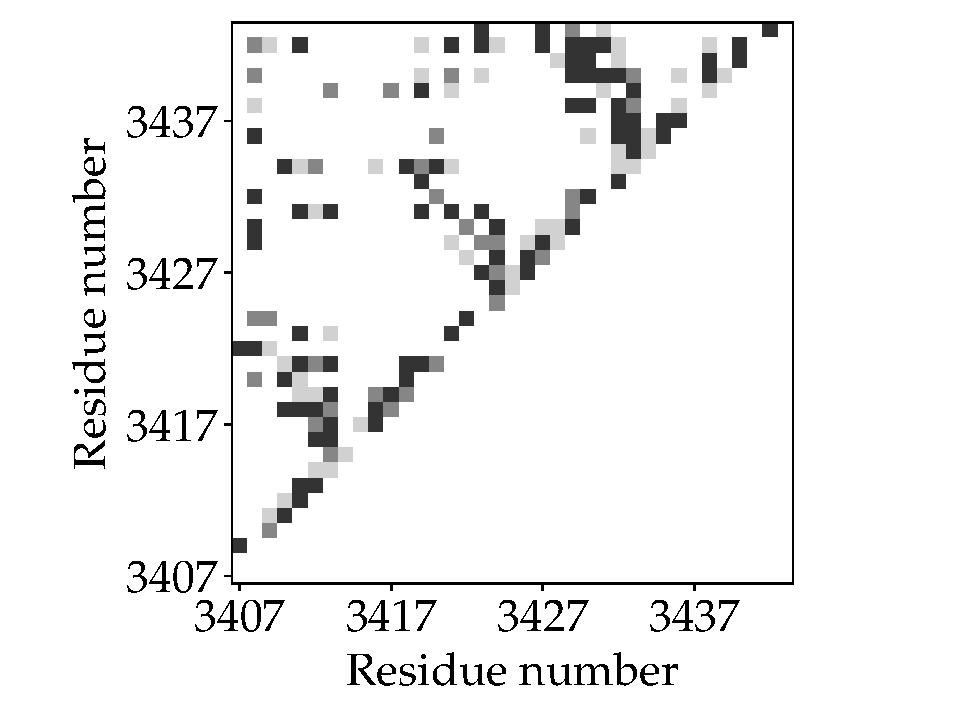
\includegraphics[trim={12mm 3mm 26mm 3mm},clip,width=0.45\columnwidth]{bioinfo/figures/beta_contactmap_base}};
    \node[anchor=south west, inner sep=0] (prot) at (2.5,0.9) {\includegraphics[width=0.2\columnwidth]{bioinfo/figures/beta_prot}};
\end{tikzpicture}
}
	\hfil
	\caption{Typical contact maps of secondary structure elements.}\label{fig:contact_patterns}
\end{figure}



\section{Assessing the field: \CASP}
The Critical Asessment of protein Structure Prediction (\CASP) is a biennial community-wide experiment to evaluate the status of the field.
Over the course of a few months, they release the sequences of around 100 unpublished structures, asking groups to predict contact maps, 3\textsc{d} models, and predicting the quality of the submissions.

This is a completely blind test.
\todo{casp}

\part{My work} \label{part:work}

\chapter{Papers included in this thesis}

\section*{Paper I}
\begin{center}
	\textsc{ProQ3D: improved model quality assessments using deep learning}
\end{center}
\noindent
In this paper, we took the same features and dataset used to develop ProQ3, but replaced the machine learning algorithm with a multi-layer perceptron.
This allows us to make full use of the whole dataset, and boosted its performance, improving the correlation between predicted and true from 0.85 to 0.90.

\section*{Paper II}
\begin{center}
	\textsc{Large-scale structure prediction by improved contact predictions and model quality assessment.}
\end{center}

\noindent
Here we present a pipeline for contact-based \emph{ab-initio} protein structure prediction.
It predicts contacts with PconsC3, folds models with CONFOLD, and selects and evaluates the accuracy using Pcons and ProQ3.
\newpage
\section*{Paper III}
\begin{center}
	\textsc{PconsC4: fast, accurate and hassle-free contact predictions}
\end{center}

\noindent
PconsC4 is a contact predictor designed to be fast and easy to use.
In order to accomplish this, the code is very optimised, requires only one MSA, and does not depend on external predictors.
Therefore, it is easy to install, deploy, and apply in large-scale studies.


\section*{Paper IV}
\begin{center}
	\textsc{A novel training procedure to train deep networks in the assessment of the quality of protein models}
\end{center}

\noindent
The power of deep learning lies in its ability to leverage the inherent structure of the data.
In this work, we show how we can take this one step further, and bake the structure of the \emph{problem} in the architecture.
We demonstrate it is a viable alternative reaching or surpassing ProQ3D's performance on the same training and test sets, but using only a subset of the inputs.

\section*{Paper V}
\begin{center}
	\textsc{Estimation of model quality accuracy in CASP13}
\end{center}

\noindent
This paper presents the results on model quality assessment of the latest edition of the blind test Critical Assessment of (Protein) Structure Prediction, CASP13,
and serves as an independent validation for the results in Papers I and IV.


\backmatter
\newgeometry{outer=24mm, inner=12mm}

{\small \raggedright
%	\printbibliography}
	\bibliography{references}}

\end{document}
